\documentclass[12pt,english]{article}
\usepackage[a4paper,bindingoffset=0.2in,%
            left=0.4in,right=1in,top=1in,bottom=1in,%
            footskip=.25in]{geometry}
\usepackage{amsmath}
\usepackage{amssymb}
\usepackage{graphicx}

\usepackage{listings}
\usepackage{color}
\usepackage{float}

\definecolor{dkgreen}{rgb}{0,0.6,0}
\definecolor{gray}{rgb}{0.5,0.5,0.5}
\definecolor{mauve}{rgb}{0.58,0,0.82}

\lstset{frame=tb,
  language=Matlab,
  aboveskip=3mm,
  belowskip=3mm,
  showstringspaces=false,
  columns=flexible,
  basicstyle={\small\ttfamily},
  numbers=none,
  numberstyle=\tiny\color{gray},
  keywordstyle=\color{blue},
  commentstyle=\color{dkgreen},
  stringstyle=\color{mauve},
  breaklines=true,
  breakatwhitespace=true,
  tabsize=3
}

\graphicspath{ {./grafice/} }

\title{Proiect SCPI\\ Instalatie nivel\\ GB76}
\date{2019\\ Decembrie}
\author{Ionescu Alexandru Cristian - 342 B3\\Pangratie Andrei - 342 B3}

\begin{document}

\maketitle
\newpage

\tableofcontents
\newpage

\section {Etapa 1}
\subsection {Initializare}

\begin{table}[H]
  \centering
  \begin{tabular}{|l|l|l|}
    \hline
    GrupID & Comanda nominala $u_0$ & Instalatie \\
    \hline
    GB76 & 55[\%] & nivel \\
    \hline
  \end{tabular}
  \caption{Date initiale}
\end{table}

\subsection {Determinați elementele de execuție si traductoarele}
\begin{figure}[H]
  \centering
    \fbox{ 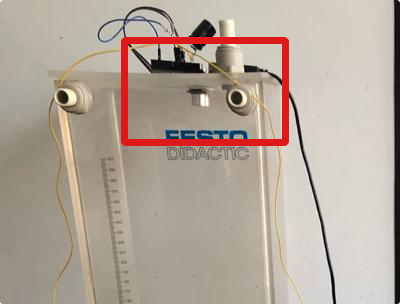
\includegraphics[width=0.6\textwidth]{instalatie_senzor.png}}
  \caption{Senzor ultrasonic de nivel}
\end{figure}

Nota: senzorul este acompaniat de o placuta Arudino pentru achizitia datelor/interpretarea lor si transmiterea catre aplicatia WinSCPI.

\begin{figure}[H]
  \centering
    \fbox{ 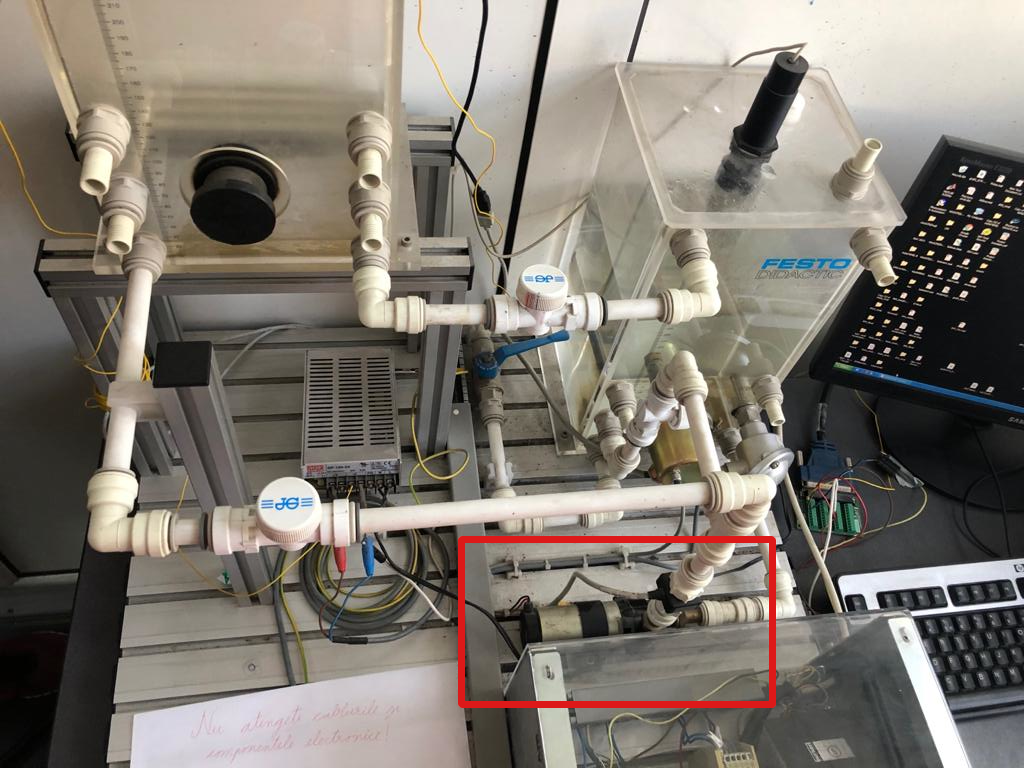
\includegraphics[width=0.6\textwidth]{instalatie_pompa.png}}
  \caption{Pompa de apa}
\end{figure}

\begin{figure}[H]
  \centering
    \fbox{ 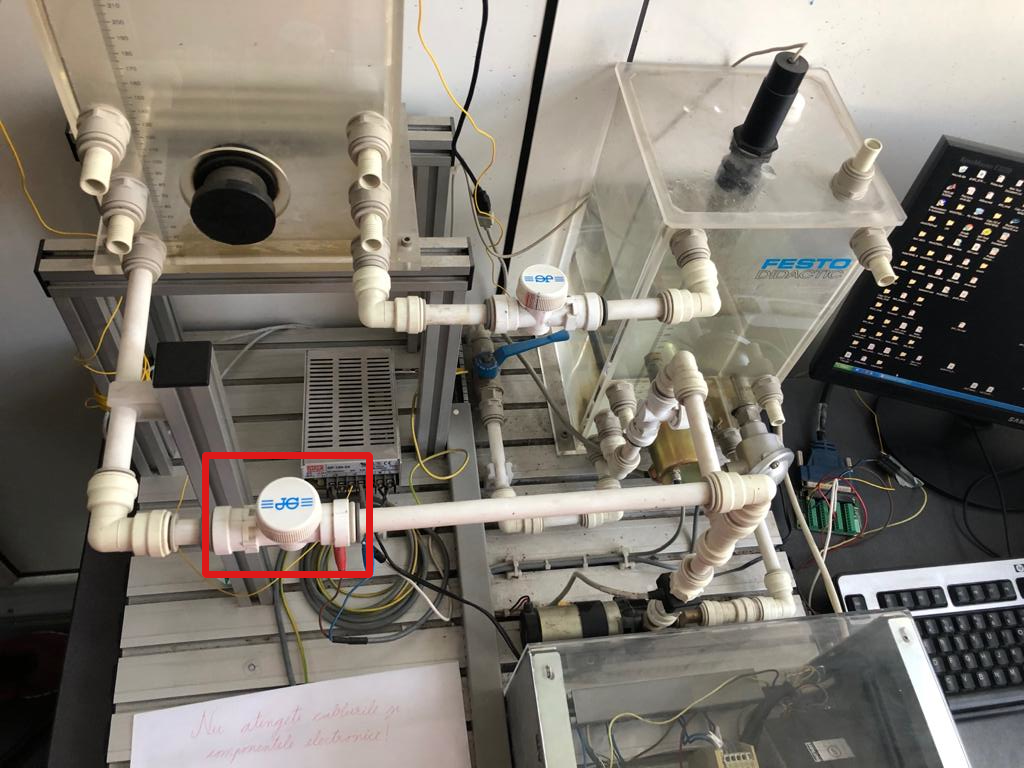
\includegraphics[width=0.6\textwidth]{instalatie_valva_in.png}}
  \caption{Valva conducta de intrare}
\end{figure}

\begin{figure}[H]
  \centering
    \fbox{ 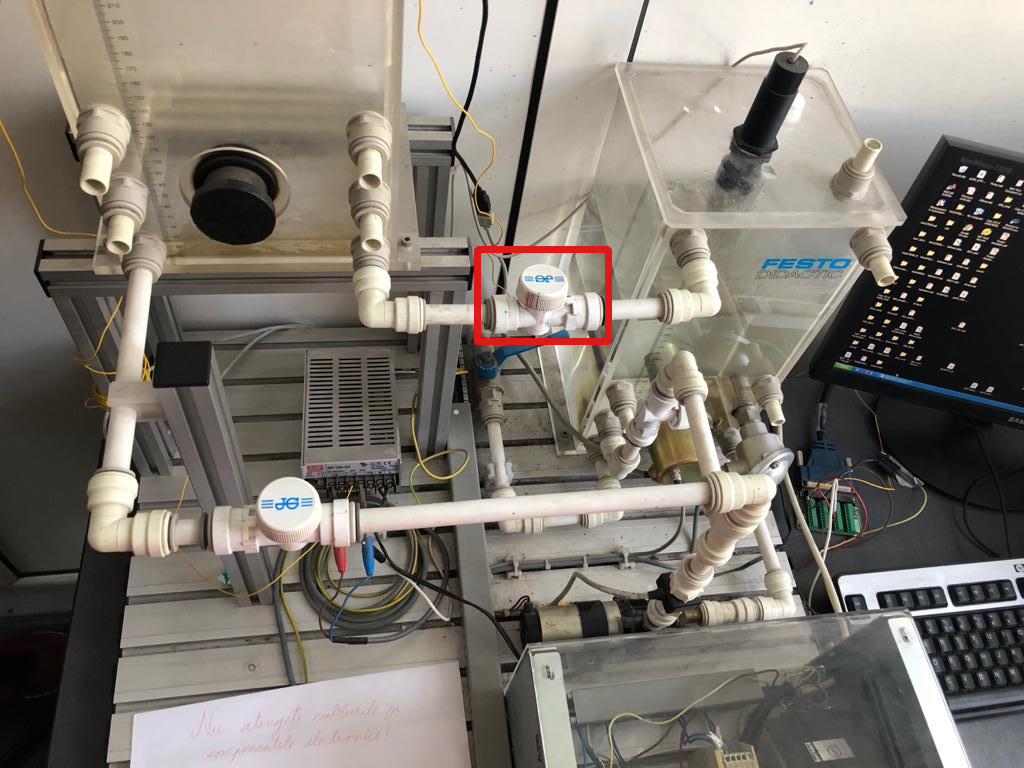
\includegraphics[width=0.6\textwidth]{instalatie_valva_out.png}}
  \caption{Valva conducta de evacuare}
\end{figure}

\begin{figure}[H]
  \centering
    \fbox{ 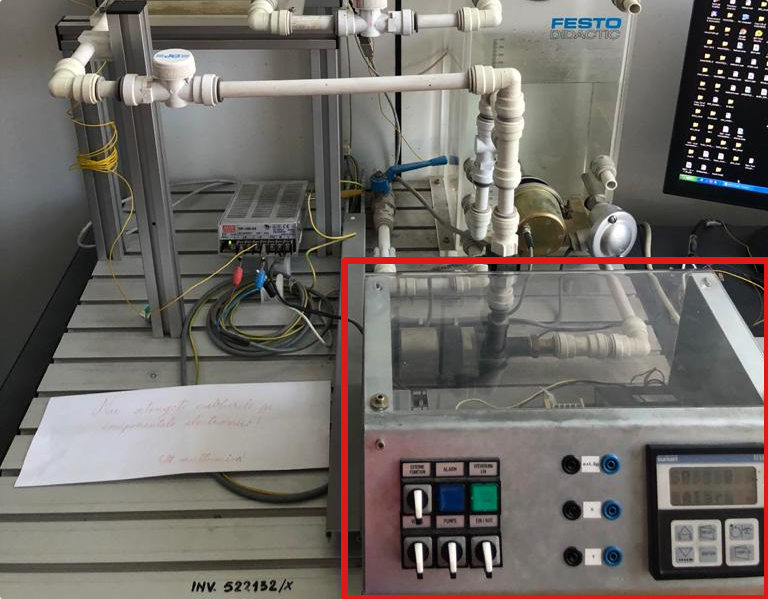
\includegraphics[width=0.6\textwidth]{instalatie_regulator.png}}
  \caption{Regulator discret}
\end{figure}


\subsection {Care este mărimea fizică care se reglează ?}
A: Inaltimea nominala a lichidului $[m]$

\subsection {Care este mărimea fizică de execuție ?}
A: Debitul de intrare in rezervor $[m^3/s]$

\subsection {Ecuația diferențială care descrie dinamica sistemului}
\begin{center}
  \begin{equation*}
  \rho F_{a}( t) -\rho F_{e}( t) =\dfrac{dM( t)}{dt} =\rho S\dfrac{dL( t)}{dt}
  \end{equation*}
\end{center}

Unde:


\subsection {Care este funcția de transfer echivalentă sistemului ?}
Sistemul poate fi echivalat cu urmatoarea functie de transfer:
\begin{center}
  \begin{equation*}
  H_{p}( s) =\dfrac{K_{p}}{T_{p} s+1}
  \end{equation*}
\end{center}

\subsection {Care sunt parametrii funcției de transfer si cum se pot determina ?}
Parametrii functiei de transfer sunt:
\begin{center}
  \begin{equation*}
  \begin{cases}
  K_{p} & Coeficient\ de\ amplificiare\ al\ sistemului\\
  T_{p} & Constanta\ de\ timp\ specifica\ sistemului
  \end{cases}
  \end{equation*}
\end{center}

Acestia se pot identifica prin mai multe metode:
\begin{enumerate}
  \item Pe cale experimentala, prin analiza raspunsului la treapta
  \item Numeric, prin liniarizarea ecuatiilor diferentiale ce descriu procesul
\end{enumerate}

In continuare, vom explora cea de-a doua metoda:


Se vor liniariza mărimile din sistem după formulele următoare:
\begin{center}
  \begin{equation*}
  \begin{cases}
  L( t) \ =\ L_{0} +\Delta L( t)\\
  F_{a}( t) =F_{a0} +\Delta F_{a}( t)\\
  F_{e}( t) =F_{e0} +\Delta F_{e}( t)
  \end{cases}
  \end{equation*}
\end{center}

Se doreste controlul nimvelului, deci in ecuatia anterioara, dupa liniarizare, trebuie inlocuit $\Delta F_e(t)$ cu dependenta fata de nivel. Pentru aceasta inlocuire se poate folosi:
\begin{equation*}
F_{e}( t) =a\sqrt{gL( t)}
\end{equation*}

Urmeaza dezvoltarea in serie Taylor:
\begin{equation*}
F_{e}( t) =F_{e0} +\left(\dfrac{\partial F_{e}}{\partial L}\right)_{L=L_{0}}\frac{( L-L_{0})}{1!} +\left(\dfrac{\partial ^{2} F_{e}}{\partial ^{2} L}\right)_{L=L_{0}}\frac{( L-L_{0})^{2}}{2!} +\ \dotsc 
\end{equation*}

Se vor face simplificari dupa liniarizare:
\begin{equation*}
( \Delta f( x))^{2} \approx 0
\end{equation*}

Se normeaza marimile de interes:
\begin{equation*}
\begin{cases}
y( t) =\frac{\Delta L( t)}{L_{0}}\\
m( t) =\frac{\Delta F_{a}( t)}{F_{a0}}
\end{cases}
\end{equation*}

Ecuatia devine in final, din care se pot identifica factorii cautati:
\begin{equation*}
T_{P}\frac{dy( t)}{dt} +y( t) =K_{P} \cdot m( t)
\end{equation*}


\section {Etapa 2}

\subsection {Configurare experiment}

Am pornit WinReg si am comutat intrerupatoarele evidentiate in imagine spre dreapta:

\begin{figure}[H]
  \centering
    \fbox{ 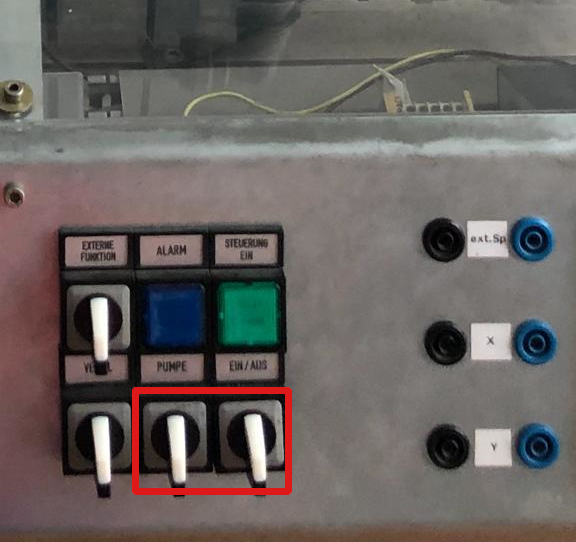
\includegraphics[width=0.8\textwidth]{instalatie_switchuri.png}}
\end{figure}

\subsection {Caracteristici proces}
\begin{table}[H]
  \centering
  \begin{tabular}{|l|l|l|l|}
    \hline
    $t_c$ & $t_t$ & $\tau$ & $T_e\ ales$ \\
    \hline
    123 [s] & 265 [s] & 12 [s] & 1 [s] \\
    \hline
  \end{tabular}
  \caption{Caracteristici proces alese experimental.}
\end{table}

\subsection {Caracteristici proces }

Am aplicat comanda nominala $u_0 = 55\%$, iar dupa am ridicat-o la $u_1 = 75\%$
\begin{figure}[H]
  \centering
    \fbox{ 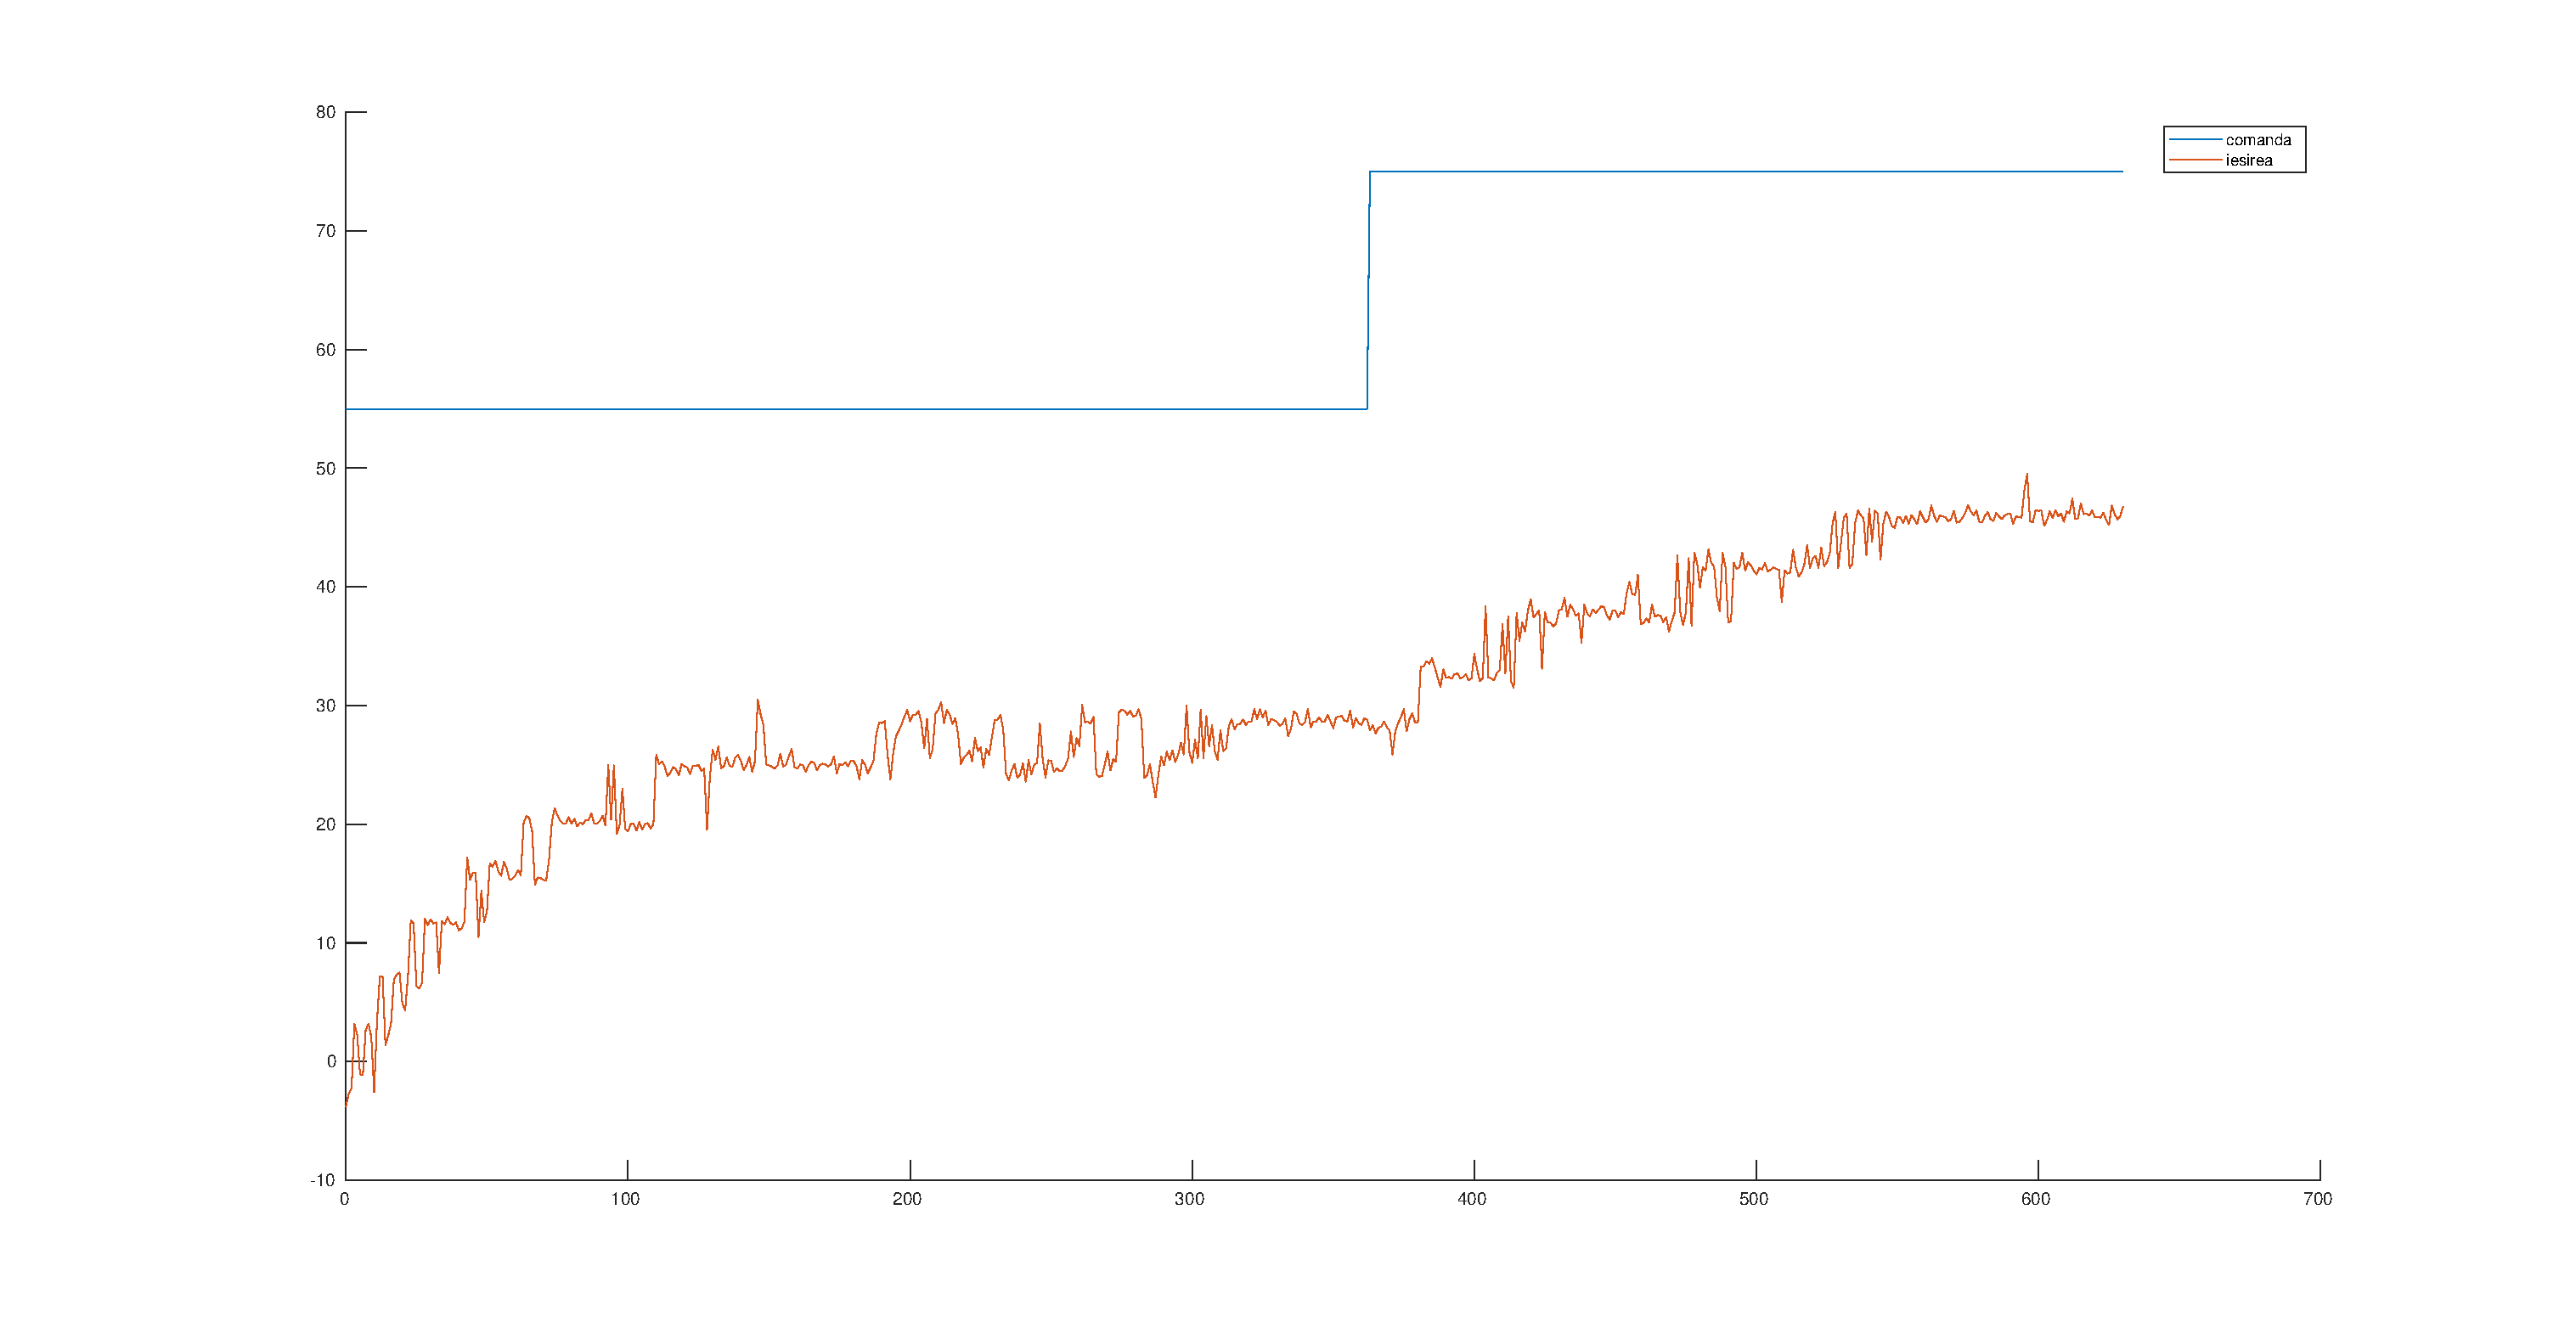
\includegraphics[width=0.8\textwidth]{2_3_1.eps}}
\end{figure}

\subsection {Model liniar}
Pe baza raspunsului la treapta, am propus urmatorul model:
\begin{equation*}
H_{F} =e^{-s\tau }\frac{K_{F}}{T_{F} s+1}
\end{equation*}

unde:
\begin{table}[H]
  \centering
  \begin{tabular}{|l|l|l|l|}
    \hline
    $\tau$ & $K_F$ & $T_F$ & $t_t$ \\
    \hline
    $12 [s]$ & $29/55$ & $160/3$ & $157 [s]$ \\
    \hline
  \end{tabular}
  \caption{Caracteristici model liniarizat.}
\end{table}

Am realizat o simulare a modelului si am suprapus-o peste datele masurate, folosite pentru identificare:

\begin{figure}[H]
  \centering
    \fbox{ 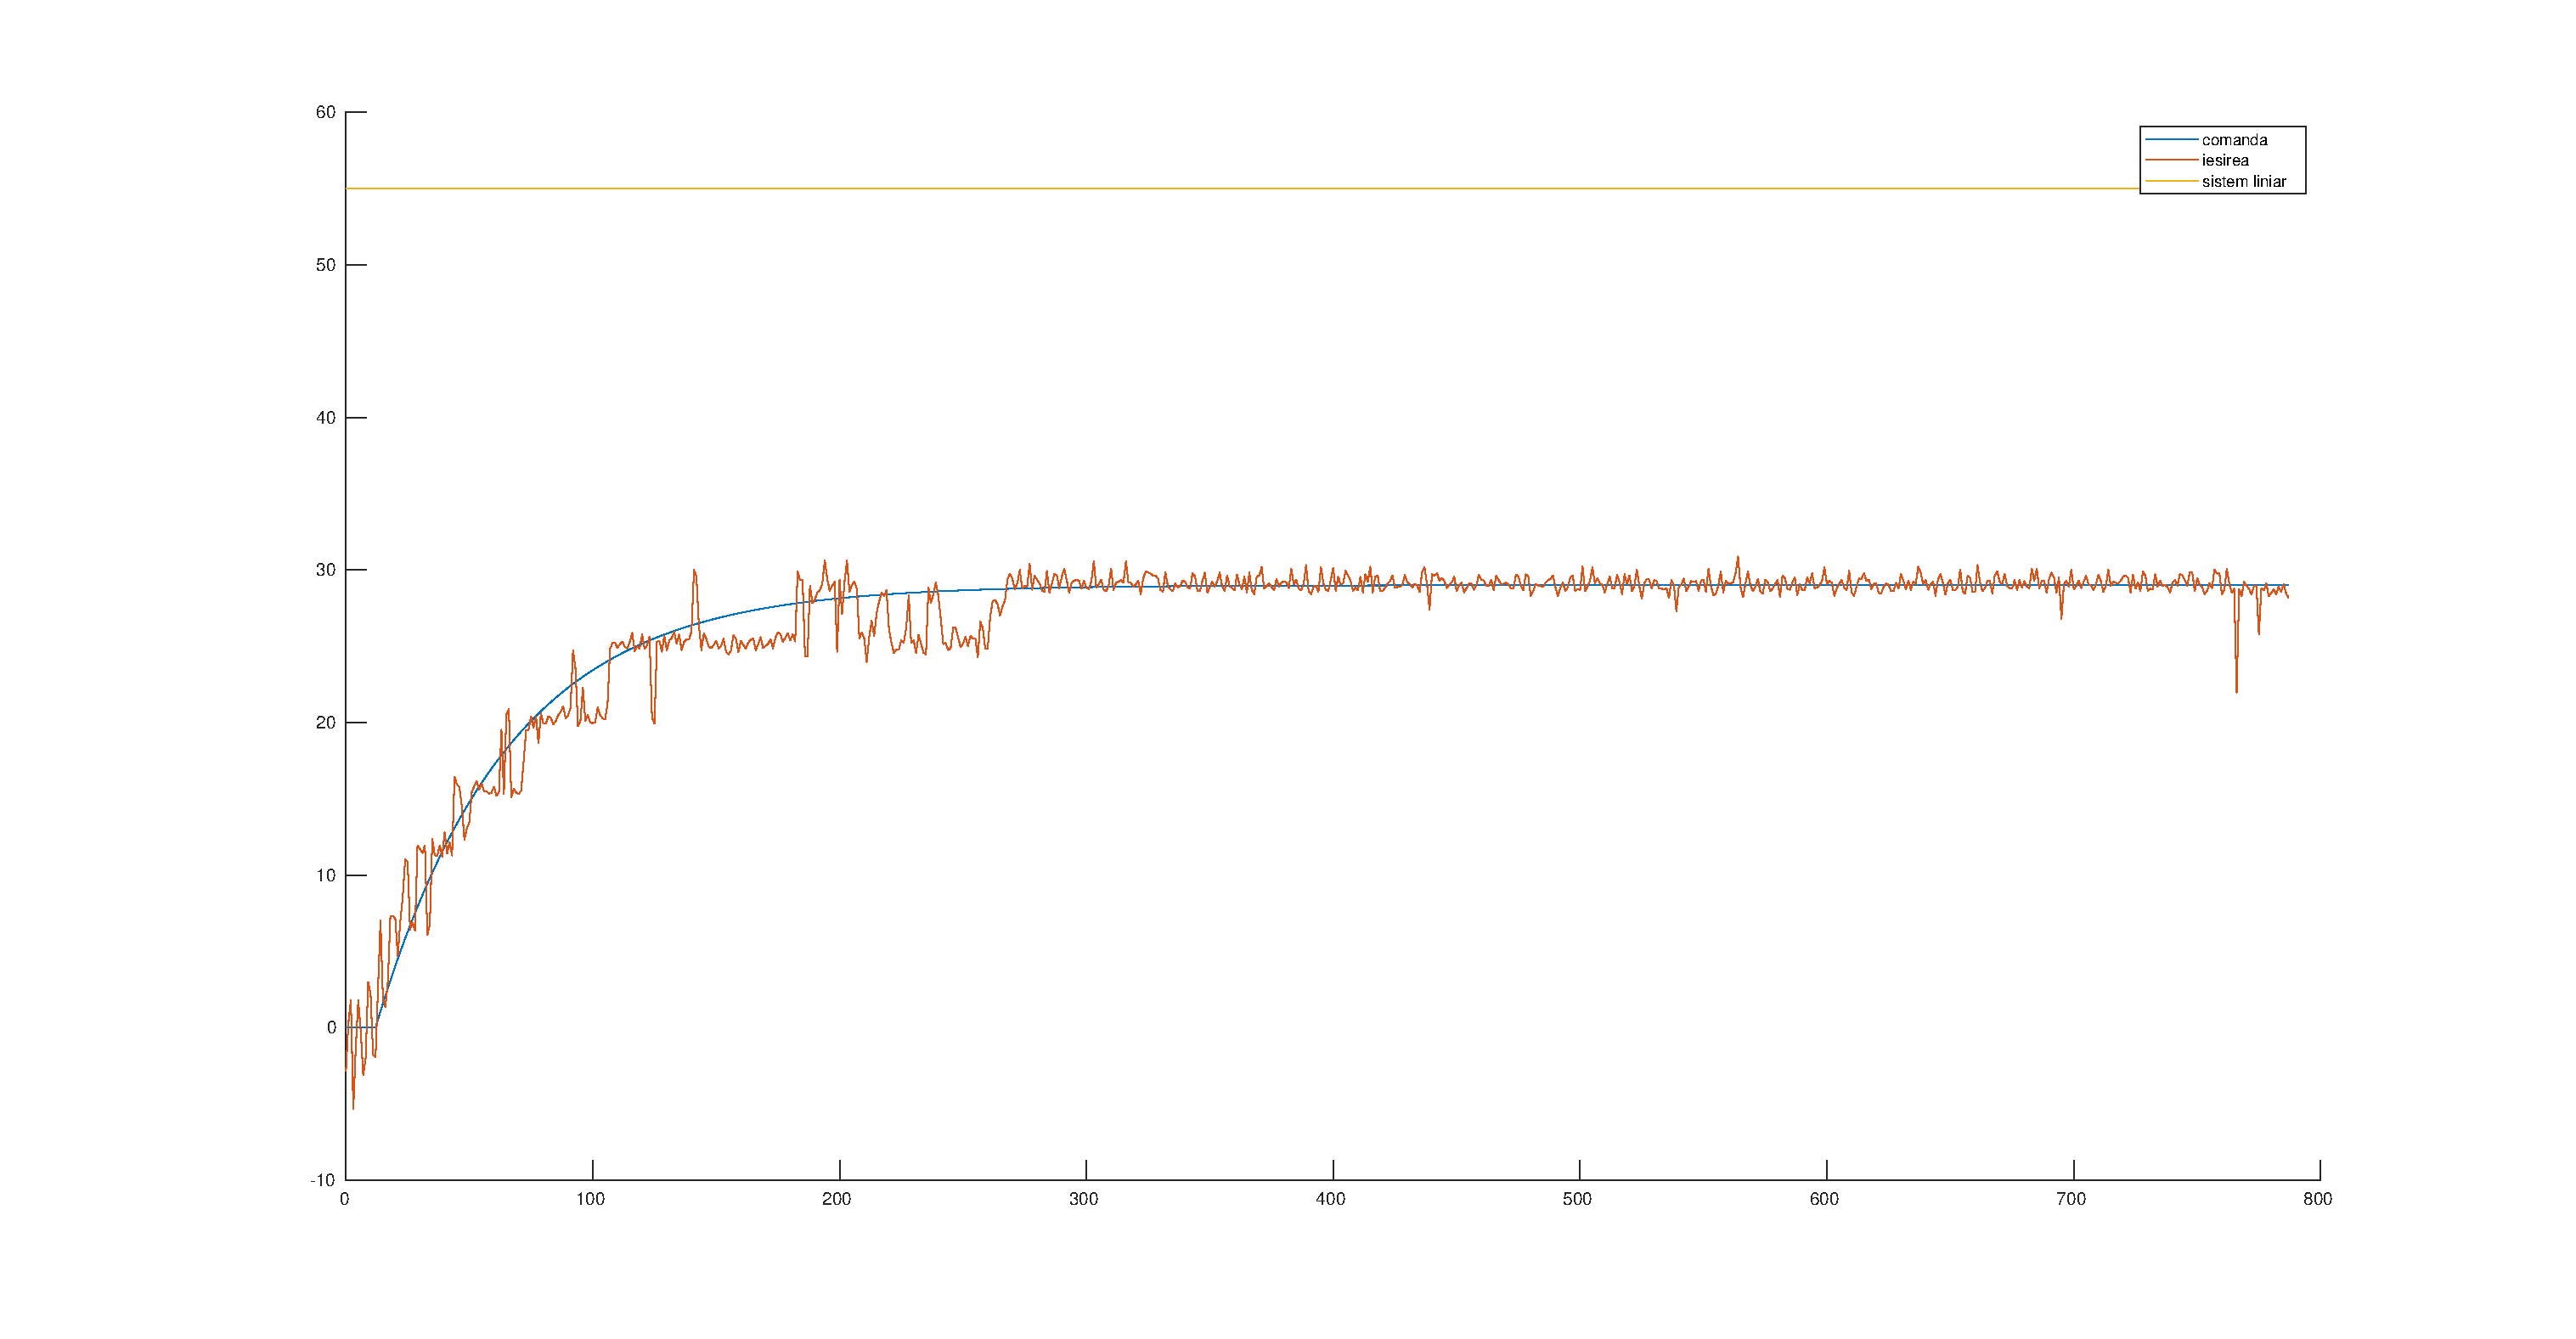
\includegraphics[width=0.8\textwidth]{2_4_1.eps}}
\end{figure}



\section {Etapa 3}

\subsection {Performante impuse}

\begin{table}[H]
  \centering
  \begin{tabular}{|l|l|}
    \hline
    $\sigma$ & $t_t$ \\
    \hline
    1.5[\%] & 198 [s] \\
    \hline
  \end{tabular}
  \caption{Performante impuse}
\end{table}

Initial am incercat acordarea cu regulator de tip Kopelovici I. Am notat factorii $K_R$ si $T_I$ obtinuti si am ajuns la concluzia ca nu satisfac performantele impuse.

Pentru atingerea performantelor impuse, am folosit un algoritm genetic si factorii anterior calculati pentru setarea limitelor de variatie ai parametrilor PID-ului.

\begin{table}[H]
  \centering
  \begin{tabular}{|l|l|}
    \hline
    $K_R$ & $T_I$ \\
    \hline
    0.9327 & 36.5748 \\
    \hline
  \end{tabular}
  \caption{Parametrii PID-ului obtinuti in urma acordarii}
\end{table}

\subsection {Simulare in continuu}

\begin{figure}[H]
  \centering
    \fbox{ 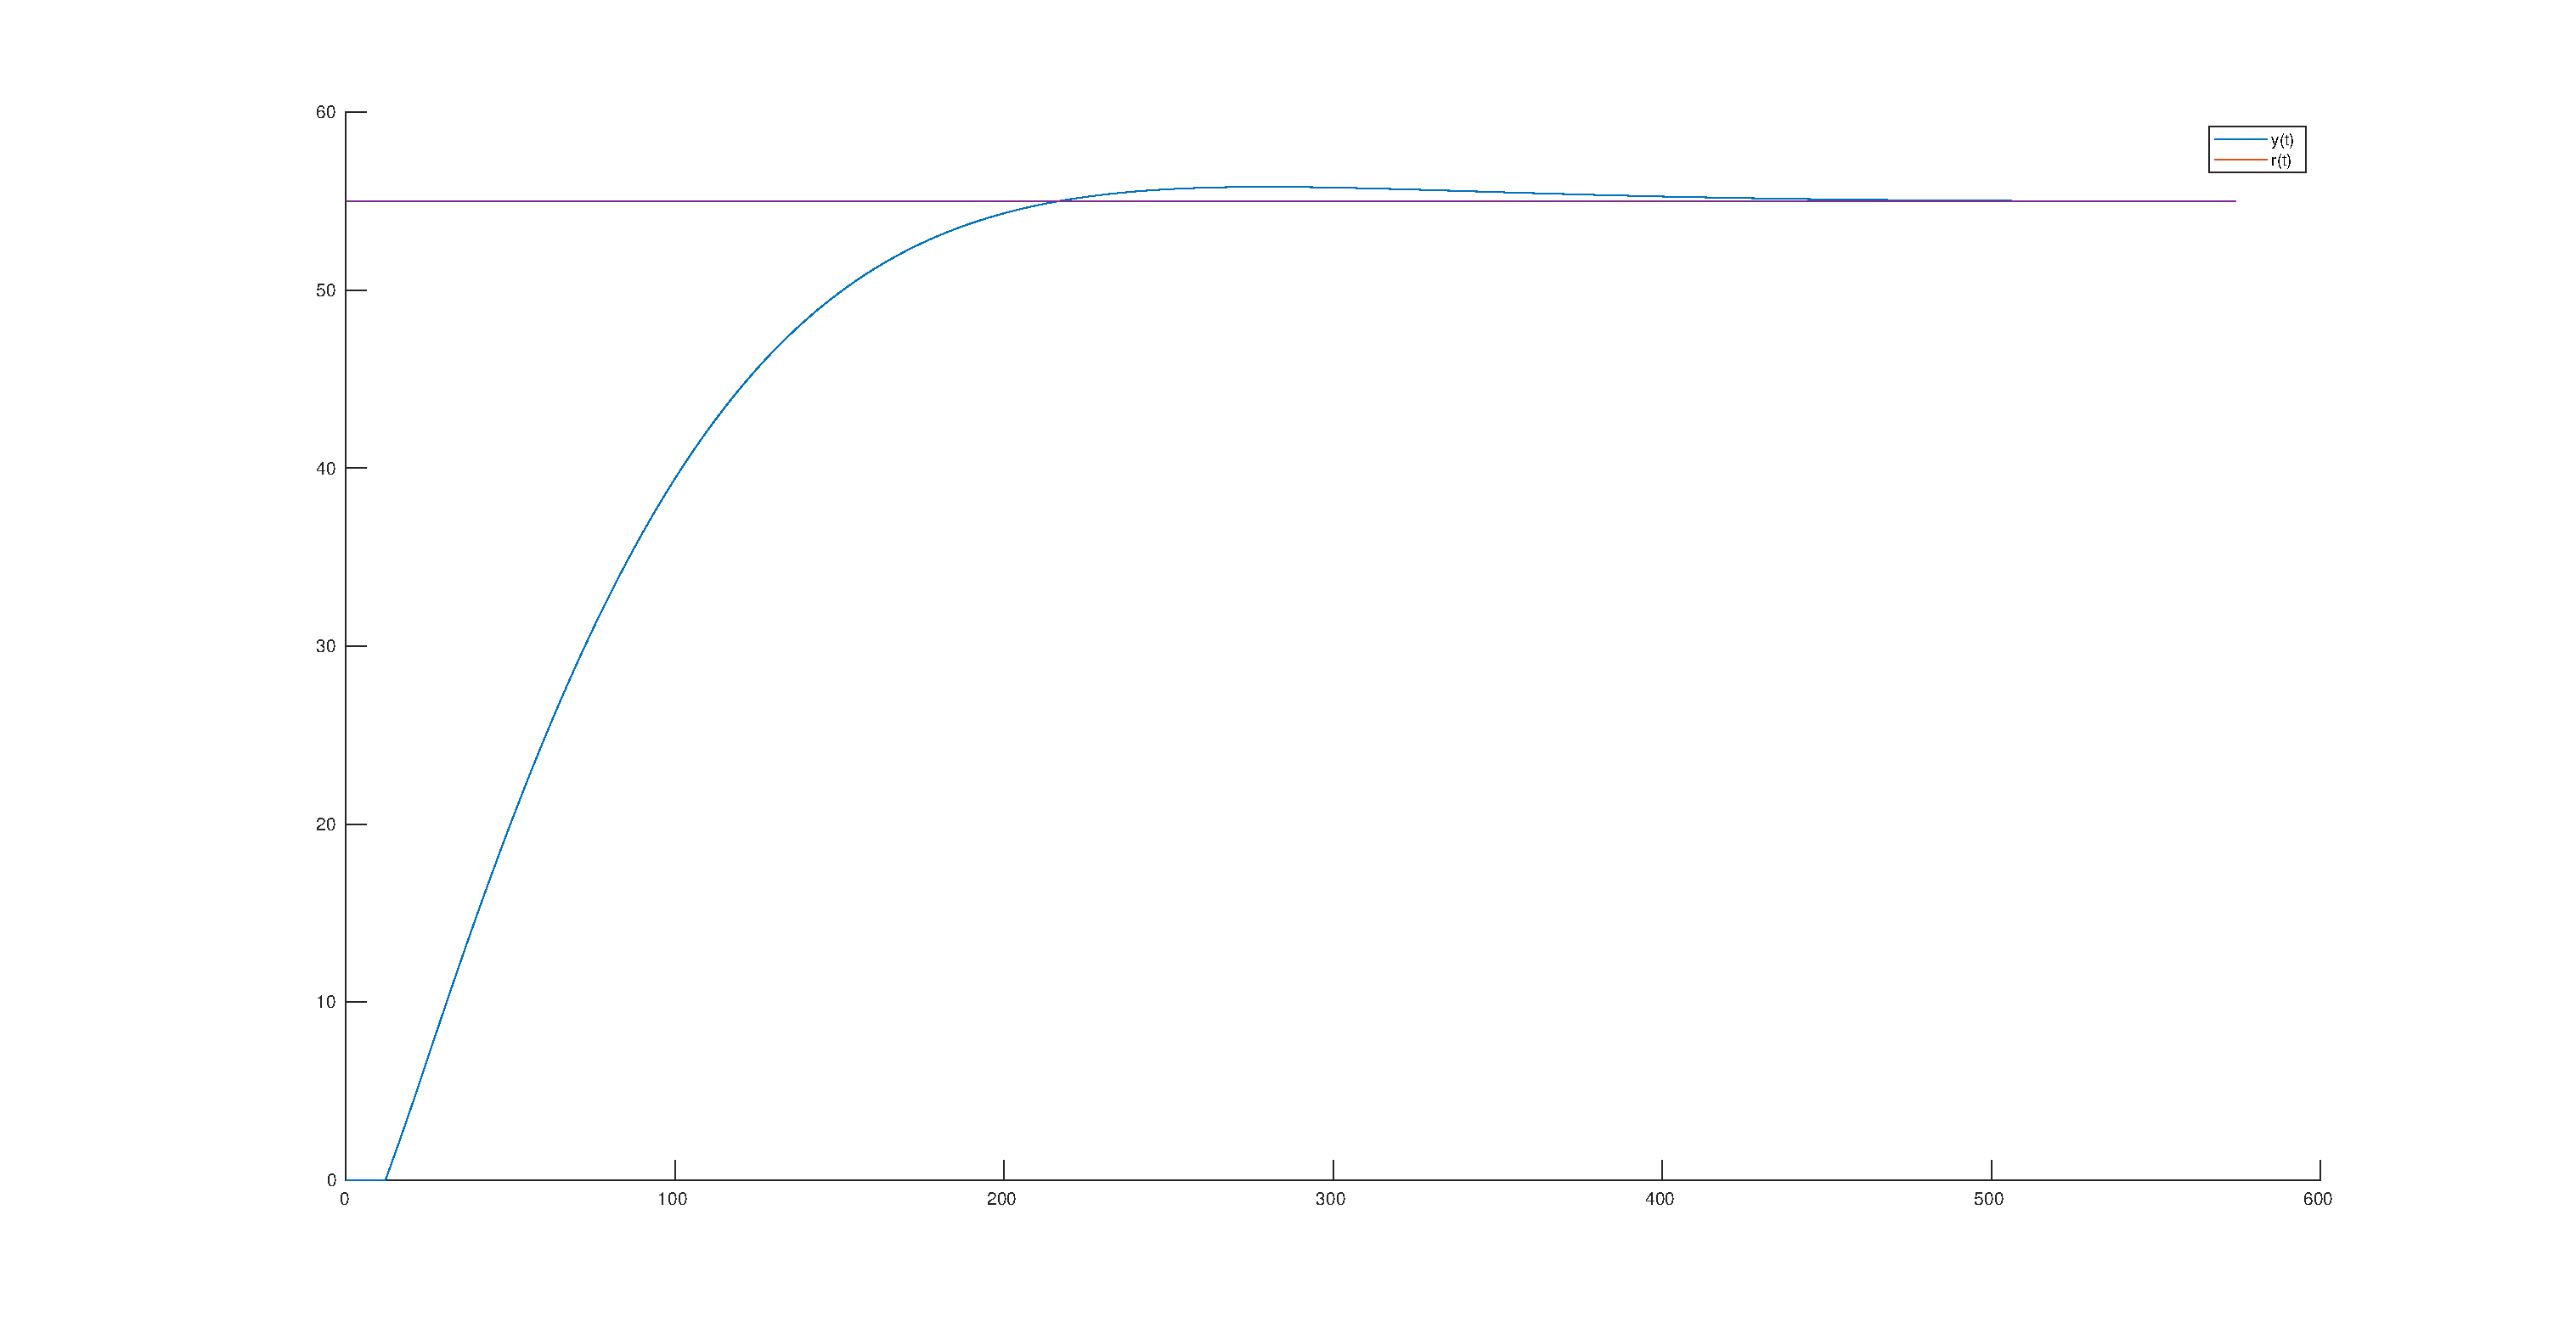
\includegraphics[width=0.8\textwidth]{3_2_1.eps}}
\end{figure}

\begin{table}[H]
  \centering
  \begin{tabular}{|l|l|}
    \hline
    $\sigma$ & $t_t$ \\
    \hline
    1.47[\%] & 192.14 [s] \\
    \hline
  \end{tabular}
  \caption{Performante obtinute}
\end{table}

Parametrii obtinuti ai regulatorului satisfac cerintele de performanta impuse

\subsection {Discretizarea legii de control}
Regulatorul obtinut prin discretizare Tustin:

\begin{equation*}
H_{R}\left[ z^{-1}\right] =\frac{0.9455-0.9199z^{-1}}{1-z^{-1}}
\end{equation*}

\subsection {Simularea regulatorului discret}

Am realizat urmatoarea schema Simulink:

\begin{figure}[H]
  \centering
    \fbox{ \includegraphics[width=0.8\textwidth]{regulator_discret.pdf}}
\end{figure}

Rezultatul simularii:
\begin{figure}[H]
  \centering
    \fbox{ 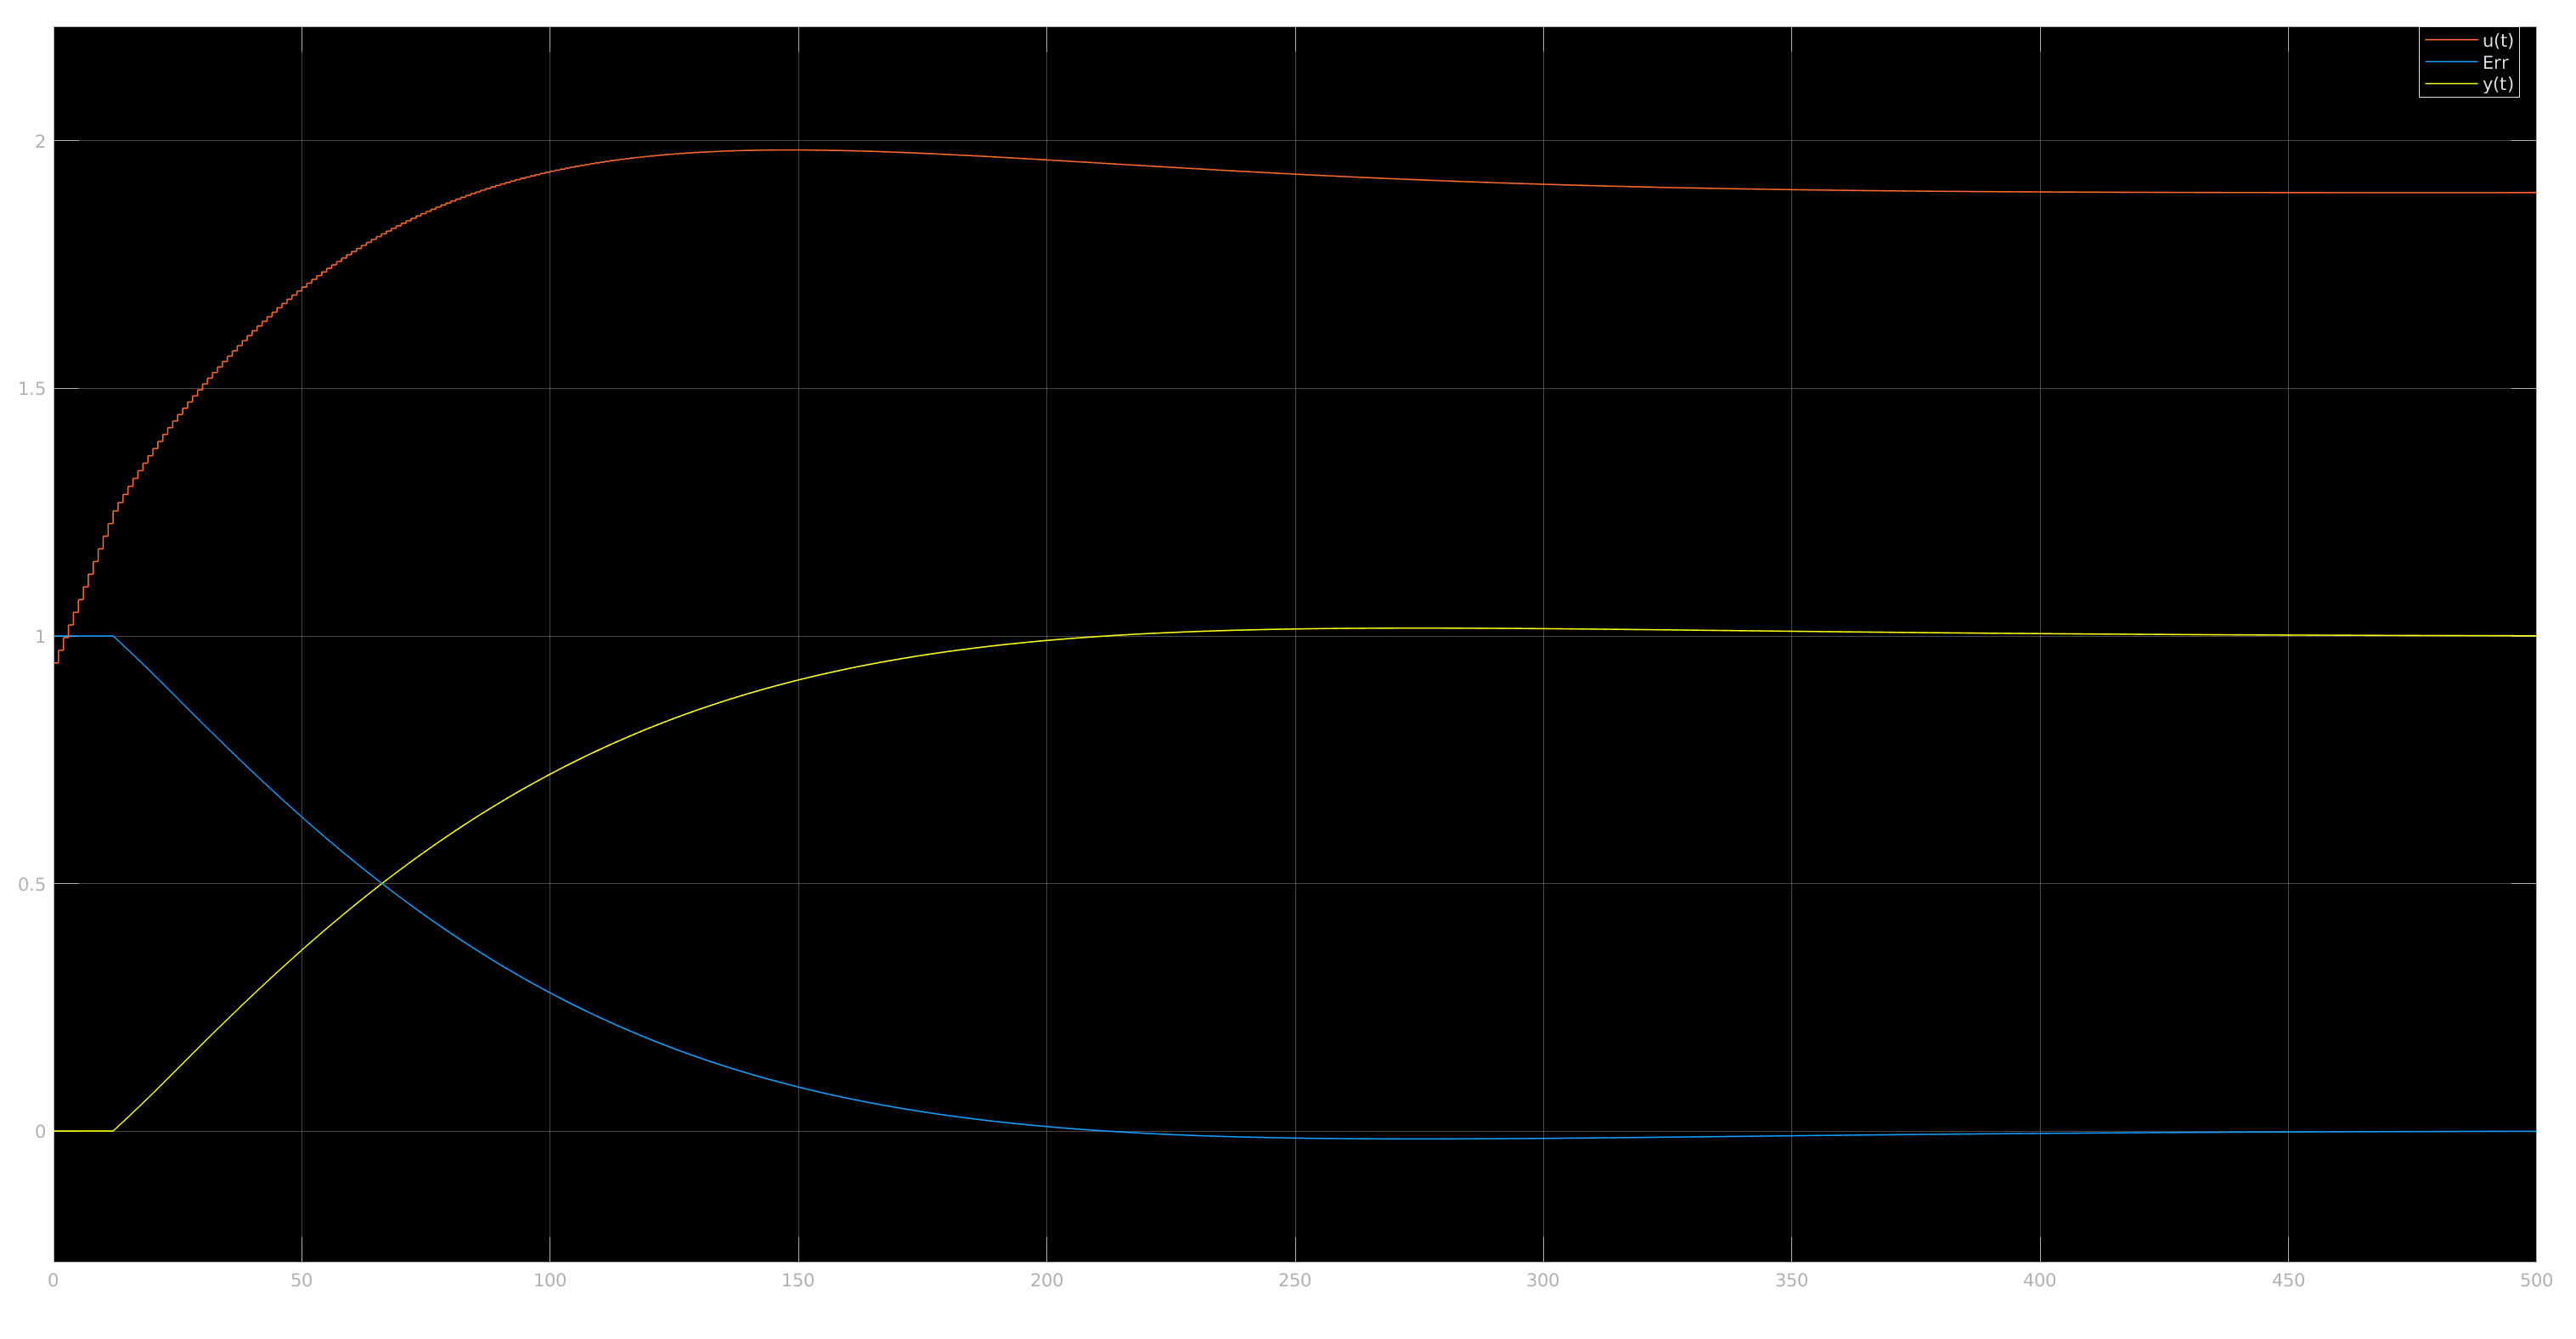
\includegraphics[width=0.8\textwidth]{3_4_1.eps}}
\end{figure}

Se observa ca regulatorul discretizat asigura performantele de reglare impuse sistemului in bucla inchisa.

\subsection {Implementarea legii de control}

Am pornit aplicatia WinSCPI si am configurat regulatorul astfel:

\begin{lstlisting}
u[k] = u[k-1] + 0.06441*(r[k] - y[k]) - 0.05226*(r[k-1] - y[k-1])
\end{lstlisting}

\begin{figure}[H]
  \centering
    \fbox{ 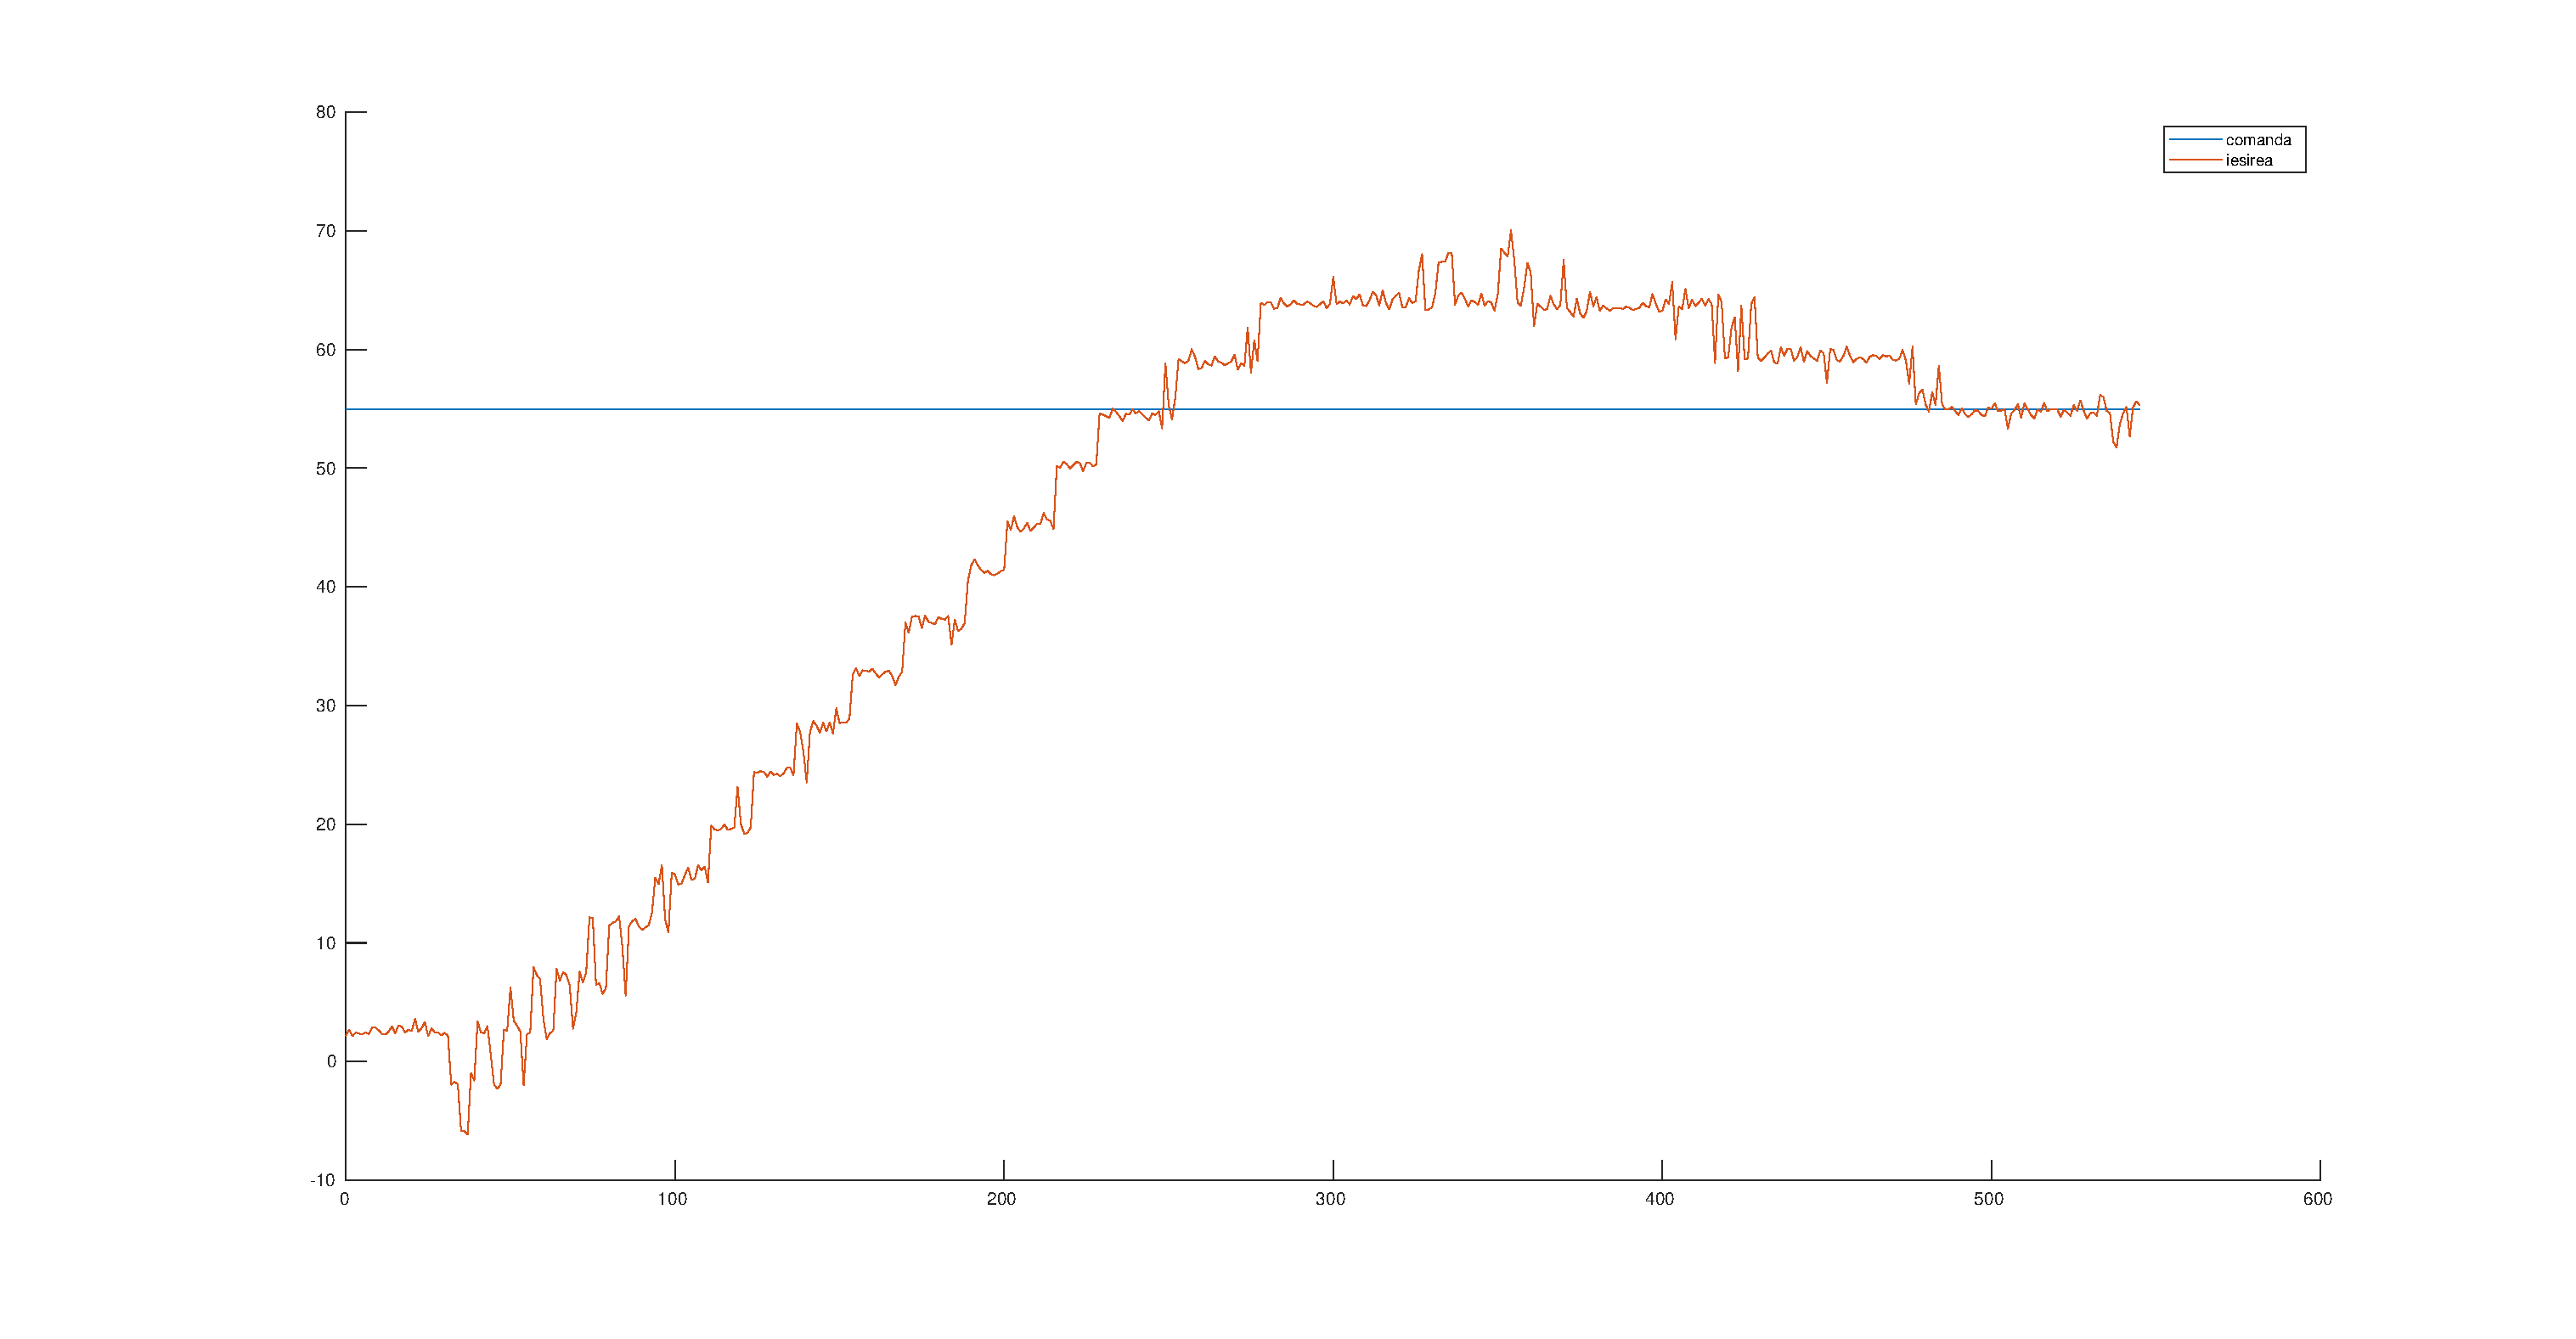
\includegraphics[width=0.8\textwidth]{3_5_1.eps}}
\end{figure}

\subsection {Concluzii}
\begin{itemize}
  \item Se observa ca overshoot-ul este mai mare in realitate
  \item Perfomantele de timp tranzitoriu sunt respectate
  \item Urmarirea referintei este asigurata ($\varepsilon _{st} = 0$)
\end{itemize}

\end{document}